\documentclass[border=10pt]{standalone}
\usepackage{tikz}
\usetikzlibrary{calc}

\begin{document}
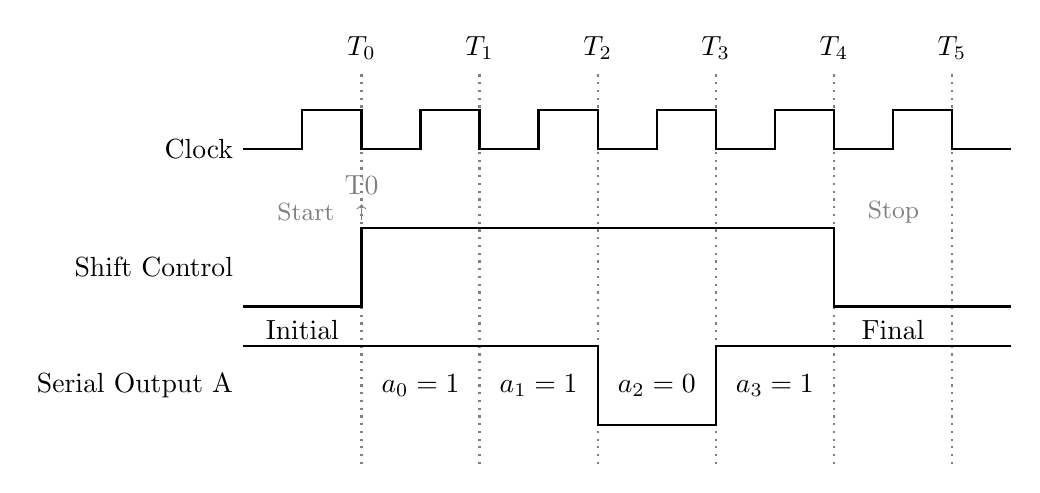
\begin{tikzpicture}[xscale=1.5, yscale=1.0, thick]
    % Time axis
    % Extend to start before T0 and end after T4
    % Range: -1 to 5
    
    % Draw Grid/Timing Lines
    \foreach \t in {0,1,2,3,4} {
        \draw[dotted, gray] (\t, -0.5) -- (\t, 4.5);
        \node[above] at (\t, 4.5) {$T_\t$};
    }
    % Add T5 line if needed, or just end
    \draw[dotted, gray] (5, -0.5) -- (5, 4.5);
    \node[above] at (5, 4.5) {$T_5$};
    
    % CLK
    \node[anchor=east] at (-1, 3.5) {Clock};
    \draw (-1, 3.5) 
         -- (-0.5, 3.5) -- (-0.5, 4.0) -- (0.0, 4.0) % Pre-T0 cycle
         -- (0.0, 3.5) -- (0.5, 3.5) -- (0.5, 4.0) -- (1.0, 4.0) 
         -- (1.0, 3.5) -- (1.5, 3.5) -- (1.5, 4.0) -- (2.0, 4.0) 
         -- (2.0, 3.5) -- (2.5, 3.5) -- (2.5, 4.0) -- (3.0, 4.0)
         -- (3.0, 3.5) -- (3.5, 3.5) -- (3.5, 4.0) -- (4.0, 4.0)
         -- (4.0, 3.5) -- (4.5, 3.5) -- (4.5, 4.0) -- (5.0, 4.0) % T4-T5
         -- (5.0, 3.5) -- (5.5, 3.5);

    % Shift Control
    % Low before T0. High T0-T4. Low after T4.
    \node[anchor=east] at (-1, 2.0) {Shift Control};
    \draw (-1, 1.5) -- (0, 1.5) -- (0, 2.5) -- (4, 2.5) -- (4, 1.5) -- (5.5, 1.5);
    
    % Serial Out FROM Reg A
    % Initial State (before T0): Reg A has 1011. Q0 is 1. So line is High.
    % T0-T1 (Shift 1): Output a0 (1).
    % T1-T2 (Shift 2): Output a1 (1).
    % T2-T3 (Shift 3): Output a2 (0).
    % T3-T4 (Shift 4): Output a3 (1).
    % After T4: Reg A restoration complete (1011). Q0 is 1. High.
    
    \node[anchor=east] at (-1, 0.5) {Serial Output A};
    
    % Waveform
    % (-1, 0): 1
    % (0, 1): 1
    % (1, 2): 1
    % (2, 3): 0
    % (3, 4): 1
    % (4, 5): 1
    
    \draw (-1, 1.0) -- (2, 1.0) -- (2, 0.0) -- (3, 0.0) -- (3, 1.0) -- (5.5, 1.0);
    
    % Labels for data
    \node at (-0.5, 1.2) {Initial};
    \node at (0.5, 0.5) {$a_0=1$};
    \node at (1.5, 0.5) {$a_1=1$};
    \node at (2.5, 0.5) {$a_2=0$};
    \node at (3.5, 0.5) {$a_3=1$};
    \node at (4.5, 1.2) {Final};
    
    % Annotations
    \node[anchor=west, gray, font=\small] at (4.2, 2.7) {Stop};
    \node[anchor=west, gray, font=\small] at (-0.8, 2.7) {Start};
    \draw[->, gray, thin] (0, 2.6) -- (0, 2.8) node[above] {T0};
    
\end{tikzpicture}
\end{document}
